\documentclass[11pt,letterpaper]{article}
\usepackage{fullpage}
\usepackage{datetime}
\usepackage[pdftex]{graphicx}
\usepackage{amsfonts,eucal,amsbsy,amsopn,amsmath}
\usepackage{url}
\usepackage[sort&compress]{natbib}
\usepackage{natbibspacing}
\usepackage{latexsym}
\usepackage{wasysym} 
\usepackage{rotating}
\usepackage{fancyhdr}
\DeclareMathOperator*{\argmax}{argmax}
\DeclareMathOperator*{\argmin}{argmin}
\usepackage{sectsty}
\usepackage[dvipsnames,usenames]{color}
\usepackage{multicol}
\definecolor{orange}{rgb}{1,0.5,0}
\usepackage{multirow}
\usepackage{sidecap}
\usepackage{caption}
\renewcommand{\captionfont}{\small}
\setlength{\oddsidemargin}{-0.04cm}
\setlength{\textwidth}{16.59cm}
\setlength{\topmargin}{-0.04cm}
\setlength{\headheight}{0in}
\setlength{\headsep}{0in}
\setlength{\textheight}{22.94cm}
\allsectionsfont{\normalsize}
\newcommand{\ignore}[1]{}
\newenvironment{enumeratesquish}{\begin{list}{\addtocounter{enumi}{1}\arabic{enumi}.}{\setlength{\itemsep}{-0.25em}\setlength{\leftmargin}{1em}\addtolength{\leftmargin}{\labelsep}}}{\end{list}}
\newenvironment{itemizesquish}{\begin{list}{\setcounter{enumi}{0}\labelitemi}{\setlength{\itemsep}{-0.25em}\setlength{\labelwidth}{0.5em}\setlength{\leftmargin}{\labelwidth}\addtolength{\leftmargin}{\labelsep}}}{\end{list}}

\bibpunct{(}{)}{;}{a}{,}{,}
\newcommand{\nascomment}[1]{\textcolor{blue}{\textbf{[#1 --NAS]}}}


\pagestyle{fancy}
\lhead{}
\chead{}
\rhead{}
\lfoot{}
\cfoot{\thepage~of \pageref{lastpage}}
\rfoot{}
\renewcommand{\headrulewidth}{0pt}
\renewcommand{\footrulewidth}{0pt}


\title{11-712:  NLP Lab Report}
\author{Rajarshi Das}
\date{\today}

\begin{document}
\maketitle
\begin{abstract}
%\nascomment{one paragraph here summarizing what the paper is about}
\noindent This is a report on the development of an open source dependency parser for the language, Bengali. I have been able to annotate a total of around 7500 tokens (around 5500 tokens for train set and 1000 tokens for each test set). The genre of the text were short stories. I have used a supervised learning approach with morphosyntactic features. The system achieves the highest accuracy of \textbf{64.39\%} on test corpus A and \textbf{66.56\%} on test corpus B. \\
\underline{Caveat:} I have used a parts-of-speech (POS) tagged dataset for my experiments. To the best of my knowledge, the data was tagged manually and hence would be highly accurate when compared to the output of an automatic POS tagger. The results of the system would be different from what I have reported, if an automatic POS tagger is used instead.
\end{abstract}

\noindent The goal of this project is to design, implement and evaluate a dependency parser for the language, Bengali (also my native language). This language is characterized by a rich system of inflections, derivation and compound formation \citep{saha2004computer,chakroborty2003uchchotoro} which makes analysis and generation of Bengali, a challenging task \citep{ghosh2009dependency}.

\section{Basic Information about Bengali}
According to \citep{ethnologue}, Bengali is an eastern Indo-Aryan Language and is native to the region of eastern south Asia. It is the official language of Bangladesh and is also spoken in the Indian state of West Bengal and parts of Tripura and Assam.\\

%
\noindent Bengali is written using the Bengali script. It has 11 vowel graphemes and 39 graphemes representing consonants and other modifiers. The script is written and read horizontally from left to right. Figure~\ref{vowels} and ~\ref{cons} show the vowels (and its  various diacritics) and consonants in the Bengali script (Image source: Internet).
\graphicspath{ {images/} }
\begin{figure}[h]
  \caption{Vowels and vowel diacritics in Bengali script.}
  \centering
  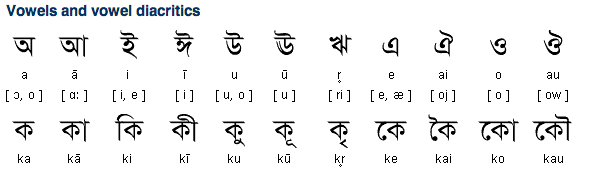
\includegraphics[scale=0.35]{vowels}
  \label{vowels}
\end{figure}
\begin{figure}[h]
  \caption{Consonants in Bengali script.}
  \centering
  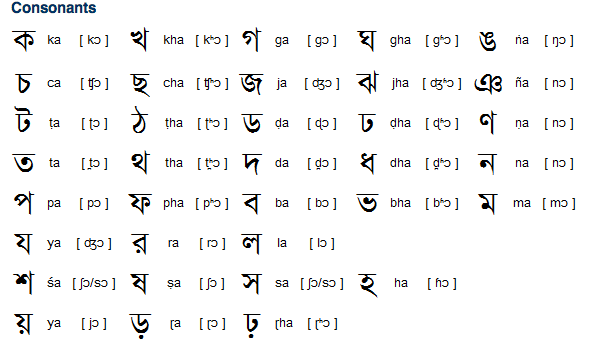
\includegraphics[scale=0.35]{consonants}
  \label{cons}
\end{figure} \\

\section{Past work on syntax of Bengali}

Bengali is a well studied language. Several work on analyzing morphology \citep{Dasgupta_morphologicalanalysis}, parts-of-speech tagging \citep{Dandapat:2007} already exists for the language in the literature. Some work has been done in building dependency parsers for Bengali. During the year 2009 and 2010, there was a shared task on dependency parsing of Indian languages  at ICON (International Conference of Natural Language Procesing). Bengali was one of the languages of the shared task.  \citep{ghosh2009dependency} have used a statistical CRF based model followed by a rule based post processing technique. \citep{Nivre_parsingindian}, \citep{ambati_09} used a transition based dependency parsing model based on MaltParser \citep{Nivre05maltparser:a}. \citep{De_Dep_ben} uses a hybrid approach where they simplify the complex and compound sentential structures and then recombine the parses of the simpler structure by satisfying the demands of the verb groups. \citep{bidir_parser} use a bidirectional parser with perceptron learning with rich context as features. \citep{kosaraju_10} used Maltparser and explored the effectiveness of local morphosyntactic features chunk features and automatic semantic information. \citep{attardi_10} used a transition based dependency shift reduce parser which used a Multi layer Perceptron classifier. They were all tested on the same dataset as a part of a shared task held at ICON 2009 and 2010. \citep{husain_09, husain_10}. In the 2009 contest, \citep{ambati_09} system performed the best and in 2010, best score of Unlabeled Attachment Accuracy was achieved by \citep{attardi_10} and the best scores for Label Accuracy and Labeled Attachment was achieved by  \citep{kosaraju_10}.

\section{Existing useful resources for the task}
 For this task, I am planning to use a dataset which was manually POS tagged. This data set was primarily used to train a statistical POS tagger. Since we are required to annotate for dependency parsing ourselves, I have decided to annotate using the manually POS tagged dataset because I think that would make the task of annotation easier. I collected the dataset from the POS tagger which is available at (\url{http://nltr.org/snltr-software/}). The dataset is a collection of short stories (with a total of around 40,000 tokens). I am also planning to use one of the freely available morphological analyzer if I plan to incorporate morphological features. 


\section{Attested phenomena in the language}
Bengali, like many Indian Languages is a free word order language. Bengali follows the SOV order in terms of ordering of subject, object and verb \citep{Dasgupta-2003}. It makes use of postpositions instead of prepositions. Determiners follow the noun while numerals, adjectives and possessors precede the noun. It exhibits no case or number agreement and no grammatical gender phenomena \citep{Dasgupta-2003}. Nouns and pronouns are declined into four cases - nominative, objective, genitive and locative \citep{Bhattacharya}. 


%There has been an annotation effort for dependency parsing in Bengali in the past as a part of the shared task held at ICON 2009 and 2010. The data was annotated using the computational Paninian Grammar \citep{Bharati}. The paninian grammatical model treats a sentence as a series of modifier- modified elements starting from a primary modified (the root of the tree - generally the main verb) \citep{Bharati-2009}. Also in \citep{Bharati-2009} and \citep{Begum-2008}, they have catalogued in detail all the annotation rules. I am planning to follow the same rules just to be consistent, so that my annotations can be reused by researchers. Although the Paninan theory was formulated by Panini (a grammarian from Ancient India) 2500 years ago for the language Sanskrit, it is basically a dependency grammar \citep{Kiparsky, Shastri}. The framework is inspired by a inflectionally rich language such as Sanskrit and gives a strong framework for annotating for other Indian Languages. Also, although \citep{Bharati-2009} has been written as a guideline for annotating Hindi treebank, similar rules should apply to Bengali, because of the similarity in the languages. 


\section{Initial Design}

For the test corpora, I have chosen one of the short story from the dataset. The short story is a conversations between few people and is characterized by lots of direct speeches and short sentences. The training corpus were also a collection of different short stories. Table \ref{Corpus_Stat} shows some statistics of the test and the train set. Since both Test A and Test B are from the same short story, there are a lot of over lapping words and therefore I expect the system's performance to  be similar on both the test corpus. Also, the text is in ITRANS format (http://en.wikipedia.org/wiki/ITRANS) instead of the native bengali script. ITRANS is an ASCII transliteration scheme for Indic scripts. There are free software packages available which converts between this format and the native bengali script. Many of the other NLP tools which I used also uses data in this format so it was easy to integrate.

\begin{table}
\begin{center}
  \begin{tabular}{ l | c | c }
  \hline
  Corpus & \#sentences & avg. \#tokens / sentence\\
  \hline
  Test A & 84 & 11.96\\
  \hline
  Test B & 97 & 10.34\\
  \hline
  Train & 571 & 10.56\\
  \hline
     \end{tabular}
\end{center}
\caption{Corpus Statstics}
\label{Corpus_Stat}
\end{table}

Next, I am going to present some of my annotation decisions. Since I don't have much experience in linguistics, some of my annotation decisions might not be correct, but for the purpose of this project I have tried to remain consistent all throughout. For doing the annotation, I have used the tool DG Annotator by Giuseppe Attardi (\url{http://medialab.di.unipi.it/Project/QA/Parser/DgAnnotator/})\\

\underline{Annotation decisions}
\begin{enumerate}
\item Multi-word names: For multi-word proper nouns, I have made the last word of the name as the root of the chunk and the tree is a linear chain with the first word being the leaf. For example, the proper noun, Mr. Ramesh Singh would become Mr $\leftarrow$ Ramesh $\leftarrow$ Singh.
\item Sometimes adverbs/adjectives are repeated in order to stress something. In this case we again form a linear chain as above. This time the root is the first occurrence of the adverb. For example. \\
\begin{center}
Aami Satyi Satyi Bolchi\\
(I)       (truly) (truly) (saying)....\\
\end{center}
In this case the two adverbs jointly form a chunk with the root as the second adverb.
\item Negative particles: In many cases, negative words normally group with the verb to change the sentence. In Bengali, the negative word usually is after the verb. I have annotated this chunk with the verb as the parent and the negative word as the child. For example. \\
\begin{center}
\underline{Karte habe} na.\\
(do)					(no)

\end{center}
 In this example, the last word (na) is a negative word and is the child of the verb to the left. 
\item In many cases, Bengali has a lot of multi verb expression (verbs occurring together to express the same thing). In such cases I have also annotated the dependency as a linear chain with the head as the first occurring verb. 
\item In Bengali, adjectives generally precede the noun. I have made the adjective as the child of the noun which it is modifying. 
\item Similar rule as above for adverbs with verbs. Sometimes the adverb and the corresponding verb are separated by few words. But in all cases the adverb is a direct child of the verb as a root.
\item Conjunctions which occur between two noun phrases have been made as the head of the two noun phrase chunks. For example, \\
\begin{center}
Tamera sa\~ Nge Chele bA meYe ....\\
(Tom)     (with)    (son)  (or) (daughter)
\end{center}
In this case the conjunction 'bA' is the head of 'Chele' and 'meYe'. 
\item For sentences which start with a conjunction, I have made the conjunction as a direct child of the root of the parse tree.
\item Bengali is characterized by `postpositions' in contrast to prepositions in English. Postpositions are made as the direct child of the nouns and pronouns it modifies (usually the noun/pronoun it follows)
\item Common nouns which occur together have also been annotated as a linear chain with the first noun as the head of the chunk. (This is a decision which I think is not grammatically sound, since I have faced some sentences where this decision was not applicable. In such cases, I have annotated the sentences in the way I felt it was correct, but I couldn't come up with a general rule for doing so)
\item The root of the sentence is usually the main verb of the sentence or a conjunction which connects two shorter sentences.
\end{enumerate}

After annotation is complete, I am planning to do supervised learning to see how the system performs. I also plan to try some unsupervised approaches such as Brown Clustering \citep{Brown92class-basedn-gram}


\section{System Analysis of corpus A}

\subsection{First round of evaluation}
I have been able to annotate around \textbf{2500} tokens in total. Separating 2000 tokens for test data, I had around 500 tokens left for training. I used the Turbo Parser \citep{MSXAF10} to train the parser. The features which I used to train the parser are POS tags (coarse and fine). The first alphabet of the POS tags are the coarse POS tags.

 The unlabeled attachment scores after training the basic, standard and full model are listed in table \ref{First}.
\begin{table}
\begin{center}
  \begin{tabular}{ l || c }
  \hline
  Model & Accuracy (\%)\\
  \hline
  Basic Model & \textbf{57.11} \\
  Standard Model & 55.59 \\
  Full Model & 55.27 \\
  \hline
   \end{tabular}
\end{center}
\caption{First round of evaluation on Corpus A. Training size of just 500 tokens}
\label{First}
\end{table}


\subsection{Performance on more training data and features}
In the few weeks, I have been able to annotate more data for training. Similar features as above were used (coarse and full POS tags). I did annotation in couple of batches. In the first batch, I annotated a total of around \textbf{3500} tokens and at the second round of effort, I was able to annotate upto \textbf{5500} tokens. Table \ref{Second} shows the unlabeled attachment scores. \\

The unlabeled accuracy scores are respectable and much better than the initial round of evaluation with just 500 tokens. It is clear that the parser was able to learn better with more training examples. On the smaller set of training examples, I got the best accuracy of \textbf{62.32 \%}. The performance of the full and the standard model were comparable. On the larger training corpus, the highest accuracy was \textbf{63.63\%} by the basic model. Also the accuracy of the full model increased to \textbf{63.19\%}, suggesting that with more training examples, it is overfitting less to the training data. On just adding more training data, the accuracy increased quite a lot. I am hoping that on Test corpus B, it is going to perform equally well or better since both the corpuses and similar and the avg. length of sentences in test corpus B is shorter as compared to corpus A. Next, I plan to try adding some more morphological features.\\

As planned earlier, I have incorporated some morphological features of the language. I have used the Bengali morphological analyzer \citep{BMA} made available by the researchers at Indian Institute of Technology Kharagpur. On manual analysis (eye-balling), the performance of the morphological analyzer looked decent.  Although there were many morphological features produced as output by the morphological analyzer, I first added the \textit{root/lemma} of a given word as one of the feature.  Table \ref{Third} (upper-half) shows the unlabeled accuracy on test corpus A. From now all the results which I will report, will all be on the larger training corpora (5463 tokens) and will have the POS (coarse and fine) tags as the feature by default. On adding lemma of the word, the performance improved!. The highest accuracy of the parser on corpus A, increased to \textbf{64.17\%} from 63.6\% by the basic model. I am a little worried that the performance of the Full model, since the performance decreased by 1\%. But since the over all performance of the parser increased, I think this feature helped.\\

Next I added, the \textit{number} and \textit{person} features with lemma. Table \ref{Third} (lower-half) shows the unlabeled accuracy on test corpus A. Interestingly, the performance of the basic model decreased to \textbf{60.91\%}. Also the accuracy of the standard and full model increased. The overall performance increased to \textbf{64.28\%}. After performing this experiment, in retrospect I realized that Bengali is a language which doesn't have any number/gender agreement. That might be one of the reason the performance of the basic model decreased so much. It does have personal pronouns and may be thats why the full and the standard model is able to learn from it.\\

In the next experiment, I threw away the number and the person features and added the \textit{tense} of the verbs. So the features now were POS tags, lemma and tense. Table \ref{Third_with_tense} (upper-half) reports the unlabeled accuracy. The performance of the basic model decreased (although not as bad as the previous experiment). The performance of the standard and the full model were moderate.\\

After these experiments, I wasn't sure which features were working the best. (I am still skeptical about the performance of the number and person features). So i thought I will include all features upto now and perform the experiments. Table \ref{Third_with_tense} (lower-half) reports the unlabeled accuracy. The basic model performs the best with an accuracy of \textbf{64.39\%}. This is also the highest accuracy received over all.

\underline{Unsupervised methods} I thought it might be a good idea to do some sort of unsupervised clustering of the words. Basically that would enable me to have a coarser representation of the words. I used brown clustering \citep{Brown92class-basedn-gram} which clusters words together having the same context. I used Percy Liang's implementation of brown clustering (https://github.com/percyliang/brown-cluster). I experimented with 100 clusters on my whole unannotated dataset (42,203 tokens). The feature which I used was the cluster number of the words. The additional features which I used are POS, lemma, tenses.  Unfortunately I didn't get any improvements. I report the results in table \ref{Unsupervised}. There wasn't any improvements in the result (although there wasn't much decrease, which I think is because of the morph features). Since the clustering approach did not look promising, I did not try any other combinations.

\begin{table}
\begin{center}
  \begin{tabular}{ l || c }
  \hline
  Model & Accuracy (\%)\\
  \hline
  Basic Model + 3641 tokens & \textbf{62.32} \\
  Standard Model + 3641 tokens & 60.48 \\
  Full Model + 3641 tokens & 60.91 \\
  \hline
  Basic Model + 5463 tokens & \textbf{63.63} \\
  Standard Model + 5463 tokens & 60.48\\
  Full Model + 5463 tokens & 63.19\\
  \hline
   \end{tabular}
\end{center}
\caption{Second round of evaluation on Corpus A.}
\label{Second}
\end{table}

\begin{table}
\begin{center}
  \begin{tabular}{ l || c }
  \hline
  Model & Accuracy (\%)\\
  \hline
  Basic Model + Lemma& \textbf{64.17} \\
  Standard Model + Lemma& 60.15 \\
  Full Model + Lemma& 62.11 \\
  \hline
  Basic Model + l + n + p& 60.91\\
  Standard Model + l + n + p& 63.30 \\
  Full Model + l + n + p& \textbf{64.28} \\
  \hline
   \end{tabular}
\end{center}
\caption{Unlabeled accuracy on Test Corpus A. Morphological features used for training.}
\label{Third}
\end{table}

\begin{table}
\begin{center}
  \begin{tabular}{ l || c }
  \hline
  Model & Accuracy (\%)\\
  \hline
  Basic Model + l + tense& \textbf{63.74} \\
  Standard Model + l + tense& 62.43\\
  Full Model + l + tense & 62.32 \\
  \hline
  Basic Model + l + n + p + t & \textbf{64.39}\\
  Standard Model + l + n + p + t & 62.11\\
  Full Model + l + n + p + t & 63.19\\
  \hline
   \end{tabular}
\end{center}
\caption{Unlabeled accuracy on Test Corpus A. Morphological features used are lemma and tenses of the verbs.}
\label{Third_with_tense}
\end{table}

\begin{table}
\begin{center}
  \begin{tabular}{ l || c }
  \hline
  Model & Accuracy (\%)\\
  \hline
  Basic Model + l + t + brown& \textbf{63.95} \\
  Standard Model + l + t + brown& 61.89\\
  Full Model + l + t + brown & 62.43 \\
  \hline
\end{tabular}
\end{center}
\caption{Accuracy on corpus A using brown clustering and some morph features (lemma, tense)}
\label{Unsupervised}
\end{table}

\section{Lessons learned and Revised Design}
The primary lessons learned from experimenting with corpus A are that more training examples improved the performance of the parser consistently. I would annotate more if I get more time, because I think it will still improve the accuracy. Also with more data the full model performs equally good as the basic model (probably will start performing better on more training data). Also adding morphological features was a good idea. I am still not sure which morphological feature is having the most difference. Since the test corpus B is similar to corpus A, I would expect similar results in them too.


\section{System Analysis of Corpus B}

I ran the same bunch of experiments on corpus B. I will report the results and my analysis for each experiments here. The first experiment was by just adding the POS tags. The results are reported in table \ref{Four} .On the smaller training corpus (3641 tokens), the highest accuracy achieved is \textbf{63.34\%} by the full model (compared to 62.32\% on corpus A). Its nice to see the full model outperforming the other models. On the larger training corpus, the results improve even further. The highest accuracy achieved is \textbf{65.45\%} again by the full model. This is significantly higher than what was achieved on the full model (63.63\%). \\

Next I experimented with the various morph features. On adding just the \textit{lemma} of the tokens, the accuracy of all the models increased!. The highest accuracy achieved here was \textbf{66.45\%} by the full model and accuracy of the basic and the standard model also increased (64.34 from 63.68 and 64.78 from 62.79) respectively. This confirms my hypothesis that morphological feature lemma was performing well. \\

The next experiment was to add \textit{number} and \textit{person} features. The results are reported in table \ref{Five} (lower-half). It is clear that adding the number and person features is decreasing performance. It supports my intuition and although this wasn't clear from the results of corpus A, it is pretty clear now. Because of the absence of number feature in bengali, the parser is not able to learn anything new or probably learning wrong things. \\

Like for test corpus A, I eliminated the number and person features and incorporated the tense feature. The results are reported in table \ref{B_with_tense} (upper-half). This improved the performance even more. The accuracy of the full model further increased to \textbf{66.56\%}. This means the morph features \textit{lemma} and \textit{tense} helps!.\\

On experimenting with every feature, the performance of the corpus decreased!. Clearly the number and person feature isn't working well. The results are reported in \ref{B_with_tense} (lower-half). 

\section{Final Revision}

Since I was annotating a linguistic task for the first time, I realized that some of the decisions which I made might not be correct and was not consistent with some of my later decisions during annotations of the training phase. So I thought I will go through the test corpus and re-annotate to be consistent with my annotations in the training set. I am reporting the results separately because according to the guidelines we were supposed to annotate the test corpus first. I report the best results which I get with each experiment for corpus A in  table \ref{revised_A} and for corpus B in table \ref{revised_B}.\\

Revising the annotations was a good idea and it is clear that it increased the accuracy. The highest accuracy achieved on Corpus A increased to \textbf{66.23\%} (from 64\%). Also this was achieved by just using the lemma and POS tags as the features (this time it outperformed the number and person feature combination). Also accuracy for test corpus B also increased to \textbf{67.66 \%} (from 66.56\%). This was achieved by the full model with lemma, POS and tense as the feature. Over all, the performances follow my prior intuition.


\begin{table}
\begin{center}
  \begin{tabular}{ l || c }
  \hline
  Model & Accuracy (\%)\\
  \hline
  Basic Model + 3641 tokens & 61.35 \\
  Standard Model + 3641 tokens & 61.90 \\
  Full Model + 3641 tokens & \textbf{63.34} \\
  \hline
  Basic Model + 5463 tokens & 63.68 \\
  Standard Model + 5463 tokens & 62.79 \\
  Full Model + 5463 tokens & \textbf{65.45}\\
  \hline
   \end{tabular}
\end{center}
\caption{Unlabeled accuracy on Test Corpus B.}
\label{Four}
\end{table}

\begin{table}
\begin{center}
  \begin{tabular}{ l || c }
  \hline
  Model & Accuracy (\%)\\
  \hline
  Basic Model + lemma & 64.34 \\
  Standard Model + lemma & 64.78 \\
  Full Model + lemma & \textbf{66.45} \\
  \hline
  Basic Model + l + n + p& 63.23 \\
  Standard Model + l + n + p& 63.01 \\
  Full Model + l + n + p& \textbf{63.79} \\
  \hline
   \end{tabular}
\end{center}
\caption{Unlabeled accuracy on Test Corpus B. Morphological features used for training.}
\label{Five}
\end{table}


\begin{table}
\begin{center}
  \begin{tabular}{ l || c }
  \hline
  Model & Accuracy (\%)\\
  \hline
  Basic Model + l + tense& 64.12 \\
  Standard Model + l + tense& 65.67\\
  Full Model + l + tense & \textbf{66.56} \\
  \hline
  Basic Model + l + n + p + t & \textbf{63.46}\\
  Standard Model + l + n + p + t & 62.35\\
  Full Model + l + n + p + t & 62.90\\
  \hline
   \end{tabular}
\end{center}
\caption{Unlabeled accuracy on Test Corpus B. In the upper half of the tables, morphological features lemma and tenses are used. In the lower-half all morphological features are used.}
\label{B_with_tense}
\end{table}
\begin{table}
\begin{center}
  \begin{tabular}{ l || c }
\hline
Model & Accuracy (\%)\\
\hline
Basic Model + POS & 65.36\\
Basic Model + POS + lemma & \textbf{66.23}\\
Full Model + l + n + p  & 65.80\\
Basic Model + l + tense & 65.58\\
Full Model + + l + n + p + t & 65.36\\
\hline
\end{tabular}
\end{center}
\caption{Accuracy on Corpus A after revised annotation on test corpus}
\label{revised_A}
\end{table}
\begin{table}
\begin{center}
  \begin{tabular}{ l || c }
\hline
Model & Accuracy (\%)\\
\hline
Full Model + POS & 66.33\\
Full Model + POS + lemma & 67.22\\
Full Model + l + n + p  & 64.23\\
Full Model + l + tense & \textbf{67.66}\\
Basic Model + + l + n + p + t & 64.12\\
\hline
\end{tabular}
\end{center}
\caption{Accuracy on Corpus B after revised annotation on test corpus}
\label{revised_B}
\end{table}

\section{Conclusion and Future work}

In this work, I have annotated dependency parse tree for around 7500 tokens (2000 for test and 5500 for training) for the language Bengali. The genre of the data was mostly short stories. I have come up with my annotation rules and have reported them. I have tried to be consistent with them, but some of these rules might not be grammatically sound. For parsing, I have used supervised approaches and have experimented using various combinations of morphological features and POS tags. The most helpful features were POS tags and \textit{lemma} of the tokens. The highest accuracy achieved on corpus A is \textbf{64.39\%} and that on corpus B is \textbf{66.56\%}. On revising the annotations for test corpus, the accuracy increased to \textbf{66.23\%} for corpus A and \textbf{67.66\%} for corpus B. 

The over all accuracy achieved by my system isn't very high and I think it can be improved by adding more training data. Also I am not very confident about the quality of my annotations and I think the performance would significantly improve if the system receives high quality annotations. Also as a future work, I would like to implement a variant of semi-supervised learning. Annotating data is very labor-intensive task but there is no dearth of unannotated data. So if we could use use the un-annotated data to improve our system, that would be great. It would be interesting to see the results of self training (testing our model on unannotated dataset and incorporating them as training data). These are some of the future extensions I would be interested in doing for improving my system.






%Therefore I trained a supervised parser (Turbo Parser) with 1000 training examples. On test dataset A (1000 tokens), it gave an unlabeled attachment score of 41.6$\%$. This is very low and I think because this is primarily because of the very less number of training examples. I plan to annotate a lot more tokens and also try to develop a rule based parser.
 

\newpage


\bibliographystyle{plainnat}
\bibliography{refs}
\label{lastpage}
\end{document}
